\section{The FSM Driver}

	The method of choice to submit the pilot to future TORCS competitions is, naturally, a \textbf{Finite State Machine}.
	A brief explanation of the behavior of this method was presented in section 2.C, for more information[2], FSMs are
	widespread over the academic knowledge in books and in the web.
	
	A race inside TORCS has some peculiarities perhaps only visible for those who possess a deeper understanding on the
	behavior of a real car, however, a layperson can absolutely develop a pilot in the environment, given the easy 
	features the interface provides. The communication between programmer and car is the main aspect that led the choice
	of a FSM for the pilot. FSMs have been one of the favorite instruments for AI gaming, and they are present in almost
	every game due to many reasons as follows:

\begin{itemize}
	\item \textbf{Readiness}: A FSM is quickly and simply implemented, in almost every one of its forms;
	
	\item \textbf{Modularity}: Debugging and reworking a FSM become catalyzed processes due to the abstraction of its
	structure, that is, its behavior can be divided into smaller, independent parts, which can be treated separately
	in a way that reduces labor;
	
	\item \textbf{Low computational complexity}: A FSM would hardly ever require great amounts of processor time, and
	that is because its operation mainly follows but hard-coded rules;
	
	\item \textbf{Intuitive behavior}: Analyzing a FSM is an easy process because human minds are often used to
	categorizing situations and conditions of conduct. This characteristic is both a good employment for debugging in
	real time and for turning the pilot's behavior simple enough so that a common person, i.e. non-programmer, could
	identify mistakes and spectate a race understanding the development of the pilot;
	
	\item \textbf{Flexibility}: A fundamental quirk of a FSM, one which makes the process of expanding the scope of the
	structure easier in a level hardly other choice of method would provide. If a new situation occurs, one that was
	not foreseen by the states defined and also one that could not be inserted in any of them, the mere creation of a
	new state would solve the matter, in about no time and almost without interference in the other parts of the whole.
\end{itemize}

The division of states for the FSMDriver itself are in agreement with the advantages of a FSM, meaning that the choice of
which states to be used relied on the human intuition of the development of a car in operation. The states designed are:

% \includegraphics[width=\textwidth]{}%
\begin{figure}[!t]
\centering
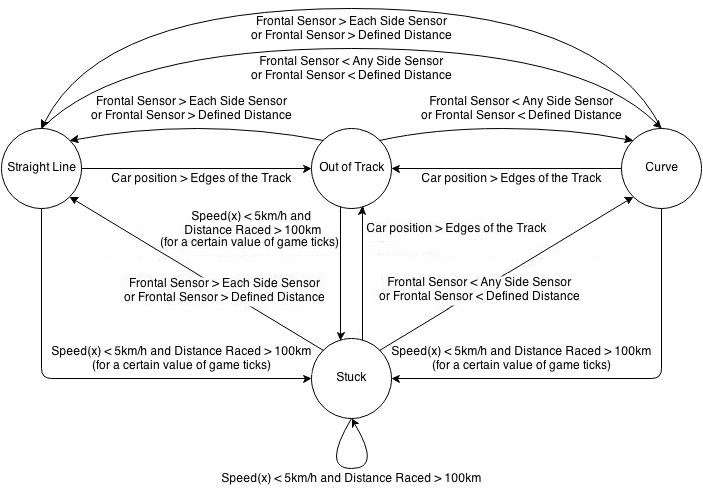
\includegraphics[width=2.5in]{StatesDiagram}
\caption{State transition diagram.}
\label{fig_sim}
\end{figure}


%\toDo{Insert image containing the proper visual state diagram image for the FSMDriver}}

\begin{itemize}
	\item \textbf{Straight line}: The state in which the pilot commands the car to full throttle and maximum 
	speed/acceleration ahead, and occurs when the car is located in a situation that sees no turning nearby;
	
	\item \textbf{Curve}: Situations focused on the steering of the car, that is, changing its direction of movement
	in order to keep it inside the delimitations of the proper racing space and also to avoid crashing the car into
	an obstacle;
	
	\item \textbf{Out of track}: When the previous states fail to prevent the car from entering an undesired situation
	such as going outside of the track, where conditions such as friction are much worse for the car than inside the
	track, this state takes control of the car and tries to return it to the race;
	
	\item \textbf{Stuck}: In a worst case scenario, when the car is barely moving, drastic measures need to be taken,
	such as reversing the car and steering it out of an obstacle. The appearence of such events reduce largely the
	performance of the pilot in the race.
\end{itemize}

In other words, the pilot will encounter four situations in a race, two of them are desired, whereas the other two are 
emergency actions. While the car is either on a \textbf{straight line} or on a \textbf{curve}, the behavior is normal; 
but when the criteria defined to manipulate the pilot into entering those states fails to keep it racing, and the car 
goes \textbf{outside of the track} or gets \textbf{stuck}, the car encounters troubles and loses performance. That is why
the accurate definition of the requirements the pilot has to fulfill to be in each of these states needs to be thought 
thoroughly for good and competitive results.
